\chapter[Results]{Simulations \& Demonstrations}
\label{cp:Results}

\parindent0pt

\section{Simulation Results}

\subsection{Simulation Setup}
\label{sec:setup}

\textbf{Implementation.} VeriFly is written in Python~3 with NumPy and SciPy (sparse-graph Dijkstra, k-d trees,
statistics), organised by responsibility into the packages of \autoref{tab:repo}. Every parameter lives in one validated configuration object that can be overridden from the
command line, for example \tcode{comms.R=30}. The test suite has 664 tests: 640 run by default in about 30\,s, and 24
slower ones check soundness under every attack. Among the most important are the decentralisation contract (no agent
imports the world), the pairing contract (paired fleets draw identical random numbers), and a cross-check of the fast
bitmask knowledge code against a textbook Kripke-model implementation.

\textbf{Visualisation.} Every mission can be exported to a self-contained Three.js web page that replays both fleets
side by side in 3D (\autoref{fig:teaser}, \autoref{fig:demo-caught}). A top-down MP4 video and a Streamlit dashboard
are also available.

\textbf{Compute.} All large experiments ran on the departmental server (3$\times$ NVIDIA RTX A5000, 40 CPU threads).
Following the lab's request not to load the CPU cores, every sweep used at most six low-priority processes
(\tcode{nice 19}), spread over the two free GPUs, with camera ray casting on the GPU.

\textbf{Baseline scenario.} \autoref{tab:baseline} lists the baseline. Each seed generates a new district: new
buildings, new collapses, new survivor positions, a new liar and new noise.

\begin{table}[!htbp]
\centering
\renewcommand{\arraystretch}{1.2}
\begin{tabularx}{\linewidth}{@{}l X l X@{}}
\toprule
\multicolumn{2}{@{}l}{\textbf{World and mission}} & \multicolumn{2}{l}{\textbf{Drones, sensing and radio}} \\
\midrule
Arena / zone   & 120\,m / 100\,m square & Fleet           & $N=10$, $F=1$, one liar \\
Coverage grid  & 2,500 cells of 2\,m    & Speed limits    & 5\,m/s horizontal, 2\,m/s vertical \\
Buildings      & 12--35\,m, 40\% collapsed & Layers / ceiling & 6, 9, 12\,m / 15\,m \\
Survivors      & 16 (70\% alive)       & Camera          & $90^\circ\times60^\circ$, 25\,m depth, 15\,m detection, 5\,Hz \\
Tick / limit   & 0.1\,s / 480\,s        & Radio           & $R=35$\,m, 10\% packet loss, 64 events/tick \\
Liar           & range-aware fake position, claims its 50\,m corner at once, from $t=12$\,s & Gate / audits & $\tau=0.3$\,s, $d_{\mathrm{safe}}=1$\,m / $q=0.1$ \\
\bottomrule
\end{tabularx}
\caption{Baseline scenario of the experiments.}
\label{tab:baseline}
\end{table}

\textbf{Statistics.} Means are reported with 95\% Student-$t$ intervals, and rates with 95\% Wilson intervals. Because
the fleets are paired by seed, naive and gated are compared with a Wilcoxon signed-rank test on the per-seed
differences. A run that has not finished when the time limit is reached is scored at the limit, which biases the
reported times of slow fleets \emph{downwards}.

\textbf{Experiments.} \autoref{tab:experiments} lists every experiment and the code state that produced it. All
numbers below are regenerated from the stored rows (\autoref{sec:code}).

\begin{table}[!htbp]
\centering
\renewcommand{\arraystretch}{1.2}
\begin{tabularx}{\linewidth}{@{}l X r l@{}}
\toprule
\textbf{Experiment} & \textbf{Design} & \textbf{Runs} & \textbf{Where} \\
\midrule
Demo mission & demo district, one blunt ambushing liar, naive vs.\ gated & 2 & local \\
\textbf{Sweep} & drones 5/10/15, liars 0/1/2, city 70/100/130\,m, one factor at a time; 20 seeds; naive vs.\ gated & 280 & server \\
\textbf{E1} four fleets & unfiltered / naive / gated / oracle, 30 districts, fair gate & 120 & server \\
\textbf{E2} detection & 4 position-lie types $\times$ whole/gradual claims $\times$ 2 fleets $\times$ 20 seeds & 320 & server \\
\textbf{E3} caution & audit fraction $q\in\{0,0.05,0.1,0.2,0.3\}$ vs.\ a coverage-only liar, 30 seeds & 150 & server \\
Localisation & W-MSR vs.\ mean, 2--8 observers, lie of 0--20\,m & 32 & local \\
2D theory studies & $\lambda_2$, Erd\H{o}s--R\'enyi robustness, degradation, trade-off (first build) & 21{,}792 & both \\
\bottomrule
\end{tabularx}
\caption[Overview of the experiments]{Overview of the experiments. E1--E3 were rerun on 11~Nov~2026 with the current
code, after an earlier round on 10~Nov with a less mature gate (590 runs), whose conclusions they confirm.}
\label{tab:experiments}
\end{table}

\subsection{Results \& Discussions}
\label{sec:results}

\subsubsection{One Mission, End to End}
\label{sec:res-demo}

We first follow a single mission on the demonstration district, in which the liar is deliberately blunt: it claims its
whole corner at once and waits in honest drones' paths. In this early demo the naive fleet ran \emph{without} the
motion gate.

\begin{figure}[!htbp]
    \centering
    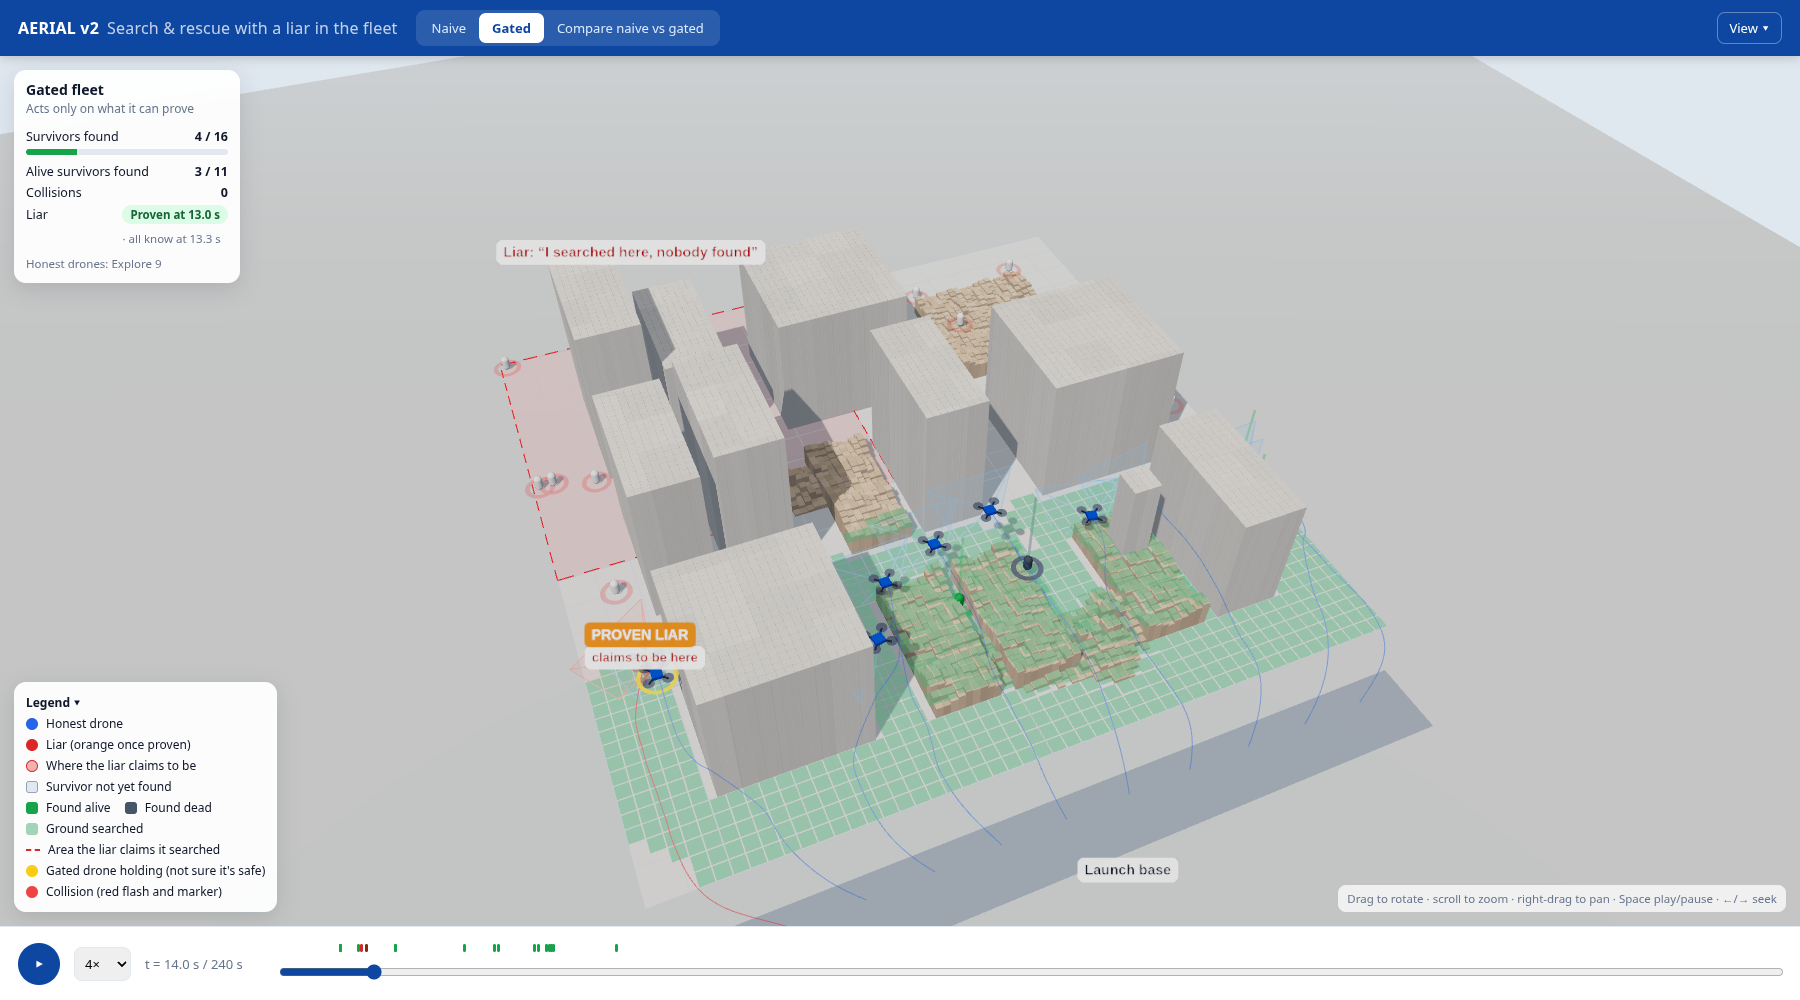
\includegraphics[width=\linewidth]{Figures/results/replay_caught.png}
    \caption[The liar is proven 0.8\,s after it starts lying]{Gated fleet at $t=14$\,s. The liar started lying at
    12.2\,s, claiming the dashed corner as searched while broadcasting a fake sweep over it (``claims to be here'').
    A neighbour compared the beacon with the UWB range of the same packet; the mismatch far exceeded $\varepsilon'$, so
    rule R1 fired at 13.0\,s. By 13.3\,s every honest drone knew the liar (orange label), and the corner had reopened
    for search.}
    \label{fig:demo-caught}
\end{figure}

\begin{figure}[!htbp]
    \centering
    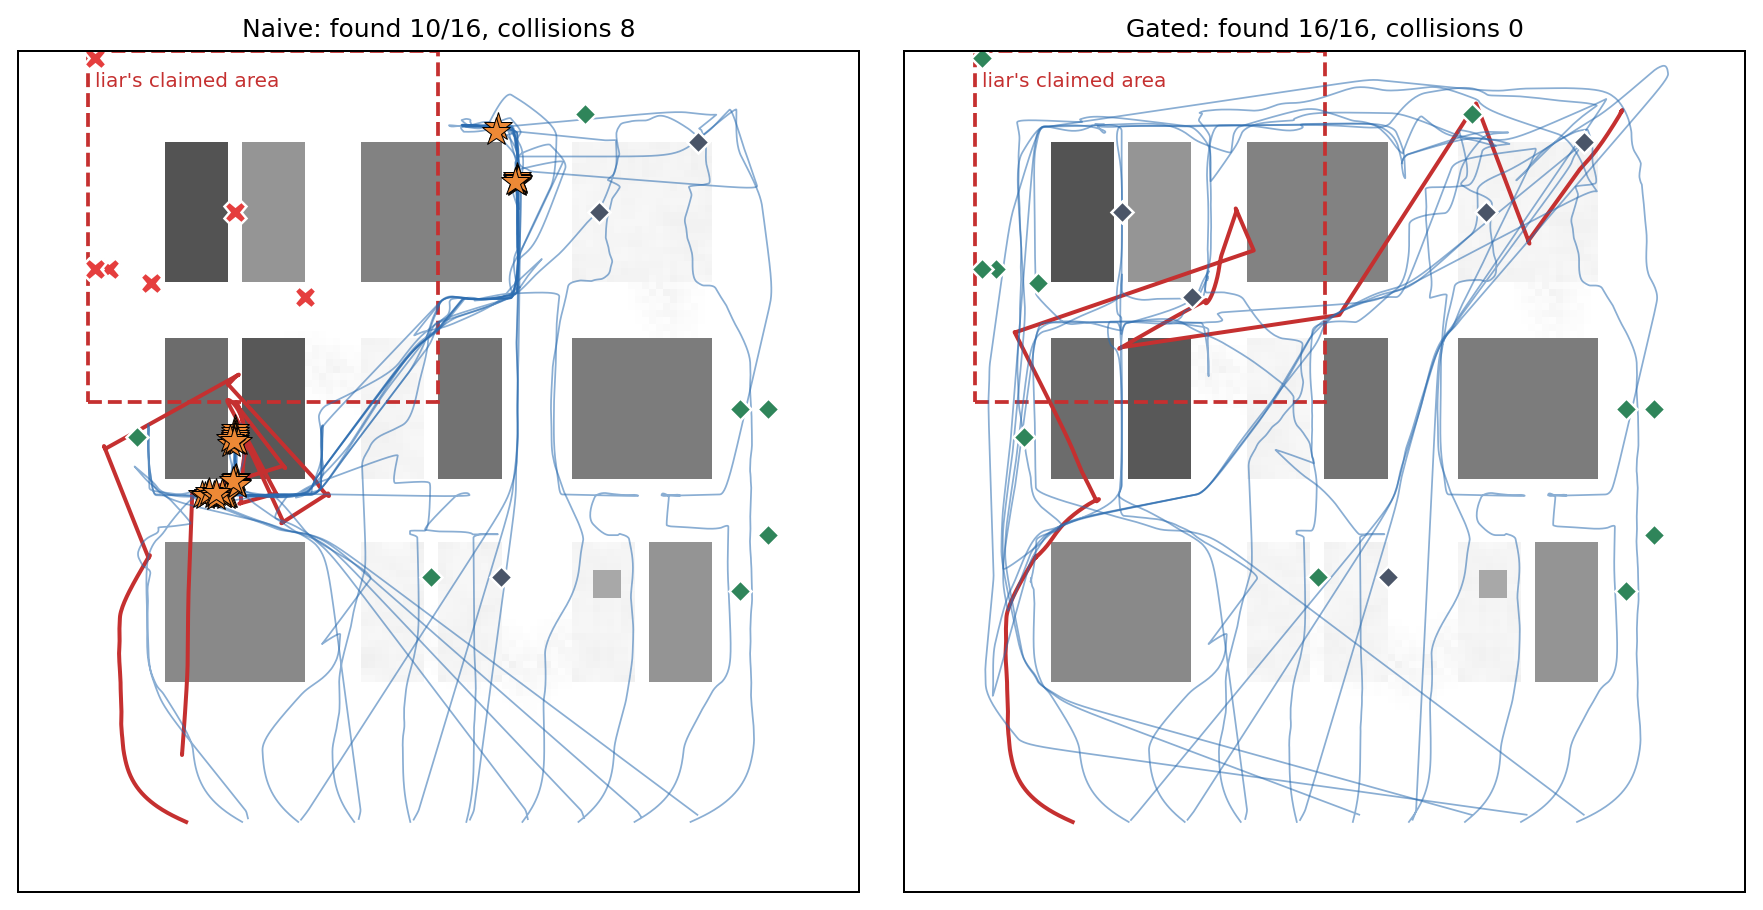
\includegraphics[width=\linewidth]{Figures/results/demo_topdown.png}
    \caption[Top-down trajectories of the demo mission]{Top-down view of the demo mission (blue: honest drones; red:
    the liar's true path). Green diamonds are survivors found alive, dark diamonds found dead, red crosses survivors
    never found, and stars are collisions. The naive fleet never enters the claimed corner and loses six survivors
    there. Its eight collisions are all between honest drones, which crowd into the remaining space without a motion
    gate. The gated fleet re-sweeps the corner and finds everyone.}
    \label{fig:demo-topdown}
\end{figure}

\begin{table}[!htbp]
\centering
\renewcommand{\arraystretch}{1.2}
\begin{tabular}{@{}l c c@{}}
\toprule
 & \naive{} & \gated{} \\
\midrule
Survivors found (alive found)          & 10/16 (7/11)  & \textbf{16/16 (11/11)} \\
Missed inside the liar's corner        & 6             & \textbf{0} \\
Collisions (pairs closer than 1\,m)    & 8 (all honest--honest) & \textbf{0} \\
First proof / all honest drones know the liar & never  & 13.0\,s / \textbf{13.3\,s} \\
All honest drones landed               & 188.9\,s      & 191.6\,s \\
False accusations                      & 0             & 0 \\
\bottomrule
\end{tabular}
\caption{The demo mission (one seed, demonstration liar).}
\label{tab:demo}
\end{table}

\autoref{fig:knowledge} makes the thesis visible. The naive fleet's \emph{believed} coverage jumps by about a quarter of
the zone the moment the liar's claim arrives; that jump is the ignorance. The gated fleet's \emph{known} coverage grows
only as fast as cells are really seen, and knowledge of the liar spreads to every honest drone within 1.1\,s of the lie.

\begin{figure}[!htbp]
    \centering
    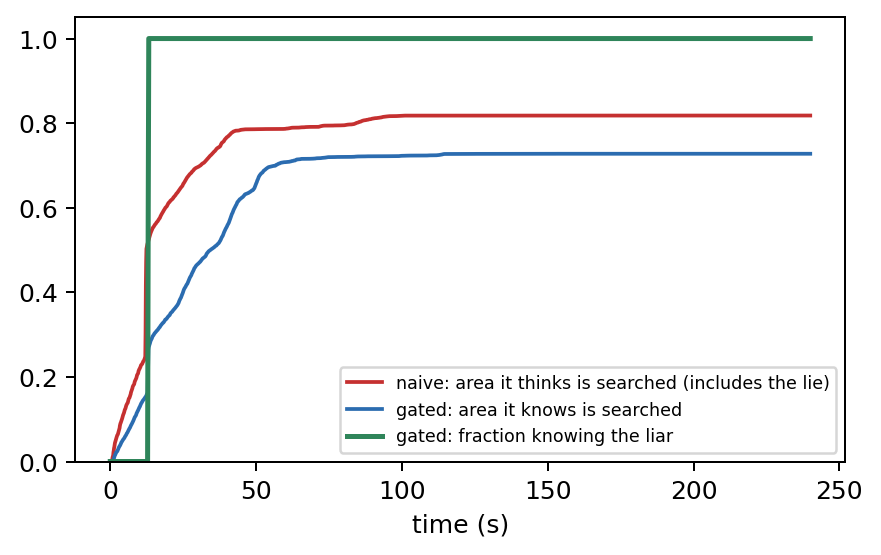
\includegraphics[width=0.72\linewidth]{Figures/results/knowledge_curves.png}
    \caption[Believed vs.\ known coverage, and knowledge of the liar]{Believed vs.\ known coverage in the demo mission
    (fractions of all 2,500 cells, including roofs that can never be searched). The step in the naive curve at 12\,s is
    the liar's false claim being accepted. The green curve is the fraction of honest gated drones that know who the
    liar is.}
    \label{fig:knowledge}
\end{figure}

\subsubsection{Parameter Sweep: Trust Costs Survivors}
\label{sec:res-sweep}

The sweep is our main experiment: 280 paired runs in which the naive fleet runs the same predictive gate as the gated
fleet but believes every report, so that \emph{trust is the only difference}. The results are in
\autoref{fig:sweep-found}, \autoref{fig:sweep-time} and \autoref{tab:sweep}.

\begin{figure}[!htbp]
    \centering
    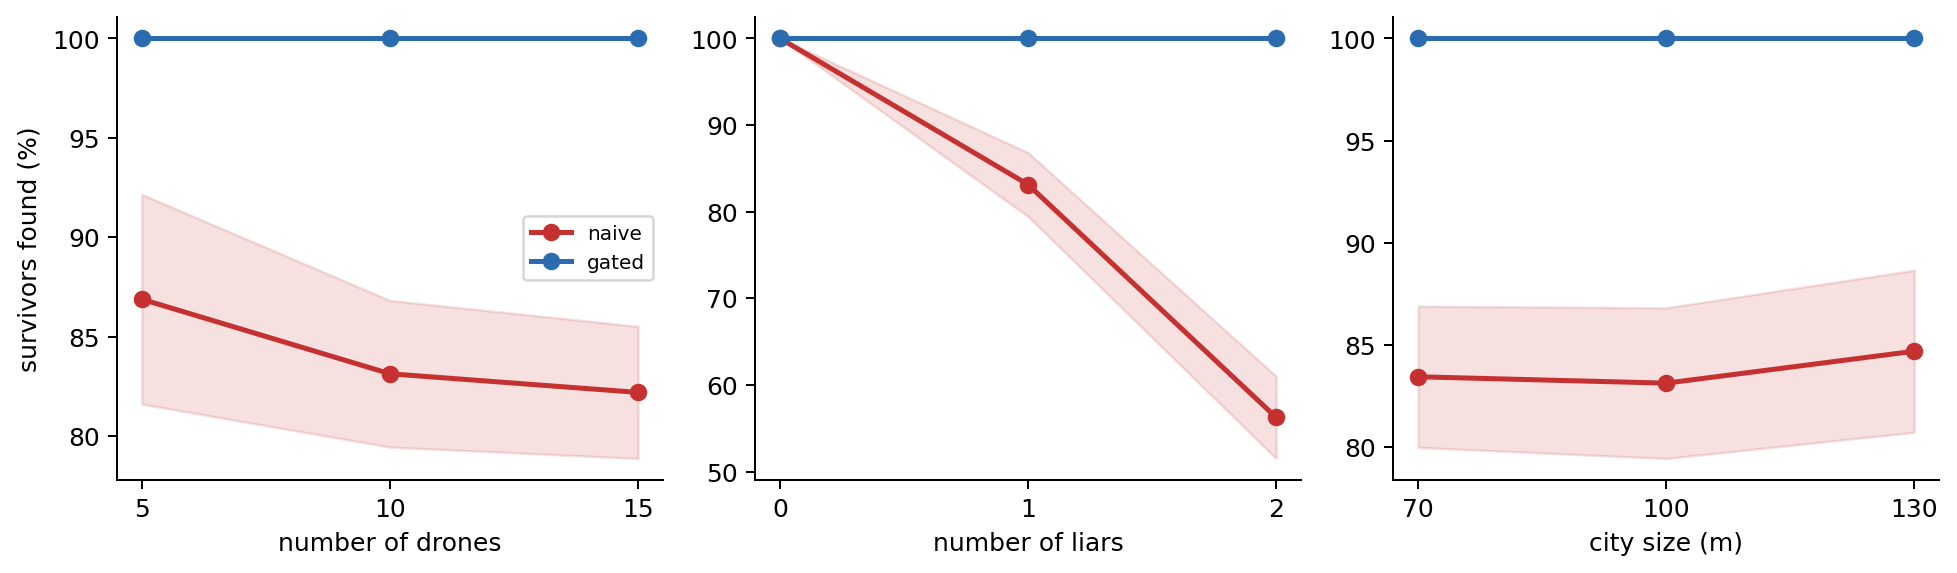
\includegraphics[width=\linewidth]{Figures/results/sweep_found.png}
    \caption[Sweep: survivors found]{Survivors found (mean of 20 paired seeds, 95\% interval shaded) when varying the
    number of drones, the number of liars, and the city size. The gated fleet finds every survivor in all 140 runs.}
    \label{fig:sweep-found}
\end{figure}

\begin{figure}[!htbp]
    \centering
    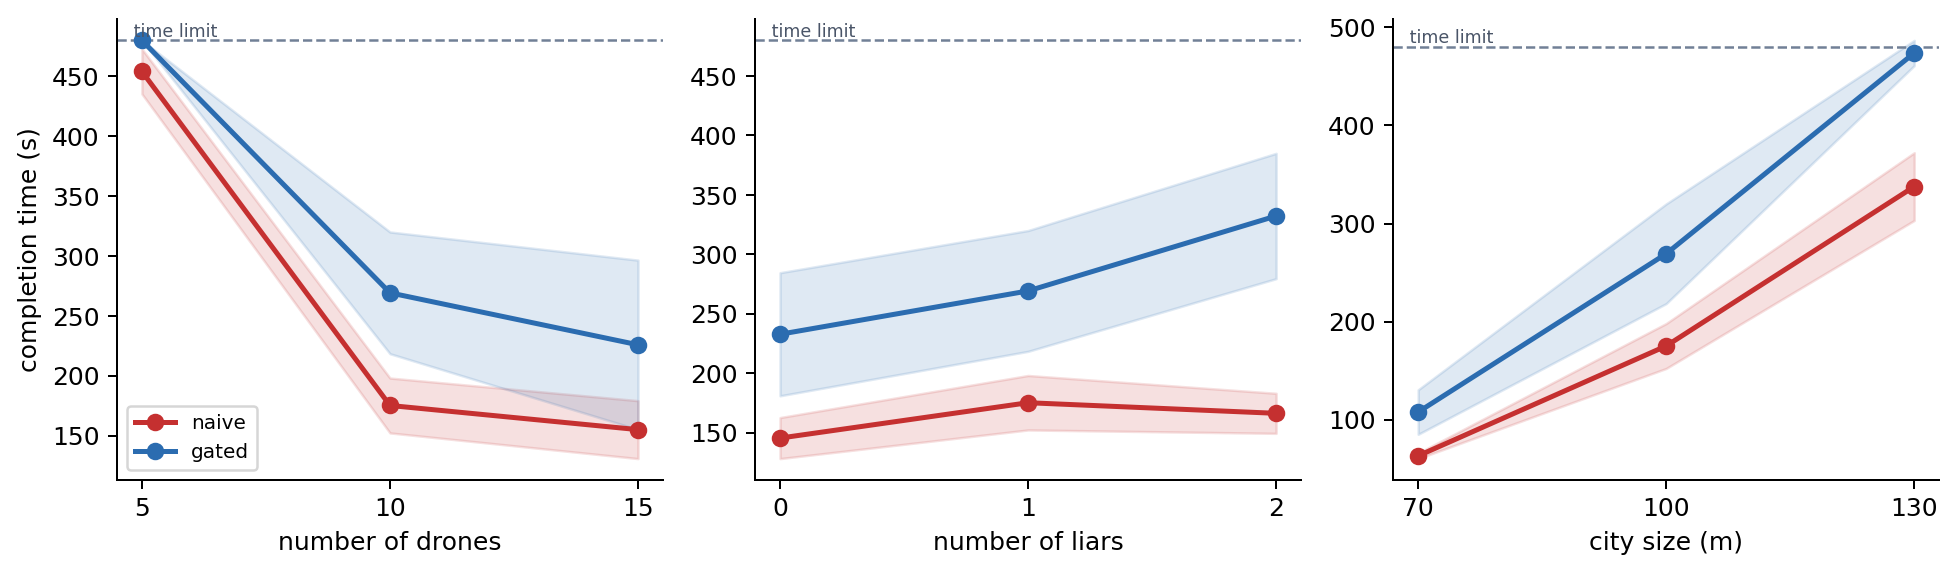
\includegraphics[width=\linewidth]{Figures/results/sweep_time.png}
    \caption[Sweep: completion time]{Completion time (all honest drones landed). Unfinished runs are scored at the
    480\,s limit (dashed), so the gated fleet's true cost with 5 drones or a 130\,m city is larger than shown.}
    \label{fig:sweep-time}
\end{figure}

\begin{table}[!htbp]
\centering
\renewcommand{\arraystretch}{1.18}
\begin{tabular}{@{}l l c c c c c c@{}}
\toprule
 & & \multicolumn{2}{c}{\textbf{Survivors found (\%)}} & \multicolumn{2}{c}{\textbf{Completion time (s)}} &
 \multicolumn{2}{c}{\textbf{Finished}} \\
\cmidrule(lr){3-4}\cmidrule(lr){5-6}\cmidrule(lr){7-8}
\textbf{Factor} & \textbf{Value} & naive & gated & naive & gated & naive & gated \\
\midrule
Drones   & 5           & $86.9\pm5.3$ & \textbf{100} & $454\pm19$ & $480\pm0$  & 50\%  & 0\% \\
         & 10 (base)   & $83.1\pm3.7$ & \textbf{100} & $175\pm23$ & $269\pm51$ & 100\% & 85\% \\
         & 15          & $82.2\pm3.3$ & \textbf{100} & $155\pm24$ & $226\pm71$ & 100\% & 80\% \\
\midrule
Liars    & 0           & 100          & 100          & $145\pm17$ & $233\pm52$ & 100\% & 95\% \\
         & 2           & $56.3\pm4.8$ & \textbf{100} & $166\pm17$ & $332\pm53$ & 100\% & 75\% \\
\midrule
City     & 70\,m       & $83.4\pm3.5$ & \textbf{100} & $63\pm3$   & $108\pm23$ & 100\% & 100\% \\
         & 130\,m      & $84.7\pm4.0$ & \textbf{100} & $338\pm35$ & $474\pm13$ & 90\%  & 5\% \\
\bottomrule
\end{tabular}
\caption[Sweep results]{Sweep results, mean $\pm$ 95\% interval over 20 paired seeds. The naive--gated difference
in survivors found is significant wherever a liar is present (Wilcoxon $p<0.002$ in every setting). The worst naive
run found 69\% of survivors with one liar and 44\% with two.}
\label{tab:sweep}
\end{table}

\begin{findingbox}[Finding 1: trust costs survivors, not collisions]
With one liar the naive fleet misses about one survivor in six in \emph{every} setting, essentially regardless of fleet
size or city size. With two liars it loses almost half. The gated fleet loses \emph{nobody} in 140 runs. Once both
fleets share the predictive safety check, collisions are rare and equal: 3 in 280 runs (two involving a liar in gated
runs, one in a naive run), with no significant difference ($p\ge0.32$; \autoref{fig:sweep-collisions}).
\end{findingbox}

\begin{figure}[!htbp]
    \centering
    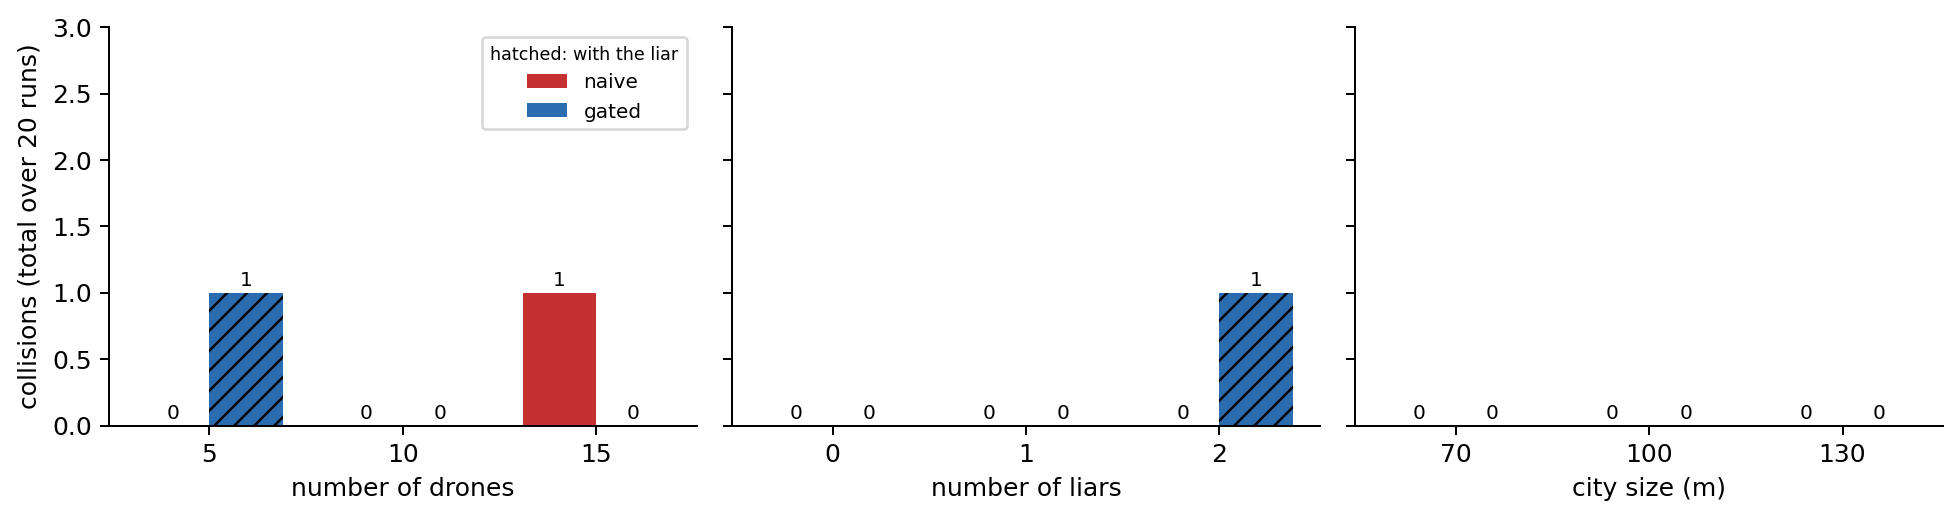
\includegraphics[width=\linewidth]{Figures/results/sweep_collisions.png}
    \caption{Sweep: collisions, totalled over 20 runs per setting (hatched: involving the liar).}
    \label{fig:sweep-collisions}
\end{figure}

\textbf{The cost of caution.} The gated fleet pays in time, about $+90$\,s at the baseline (269 vs.\ 175\,s,
$p=0.002$). Most of it is paid \emph{even with no liar} ($+87$\,s, $p<0.001$): it is the price of \emph{caution}
(holding when a move cannot be proven safe, flying only through space seen by itself or a known-honest teammate, and
auditing), not of uncertainty about who the liar is. The cost grows with
the work per drone: with 5 drones or a 130\,m city the gated fleet rarely finishes within 480\,s, while with 15 drones
the time gap is no longer significant ($p=0.19$). \autoref{fig:sweep-tradeoff} summarises the trade-off: every arrow
goes from the naive to the gated fleet on the same setup, always up (more survivors) and to the right (more time).

\begin{figure}[!htbp]
    \centering
    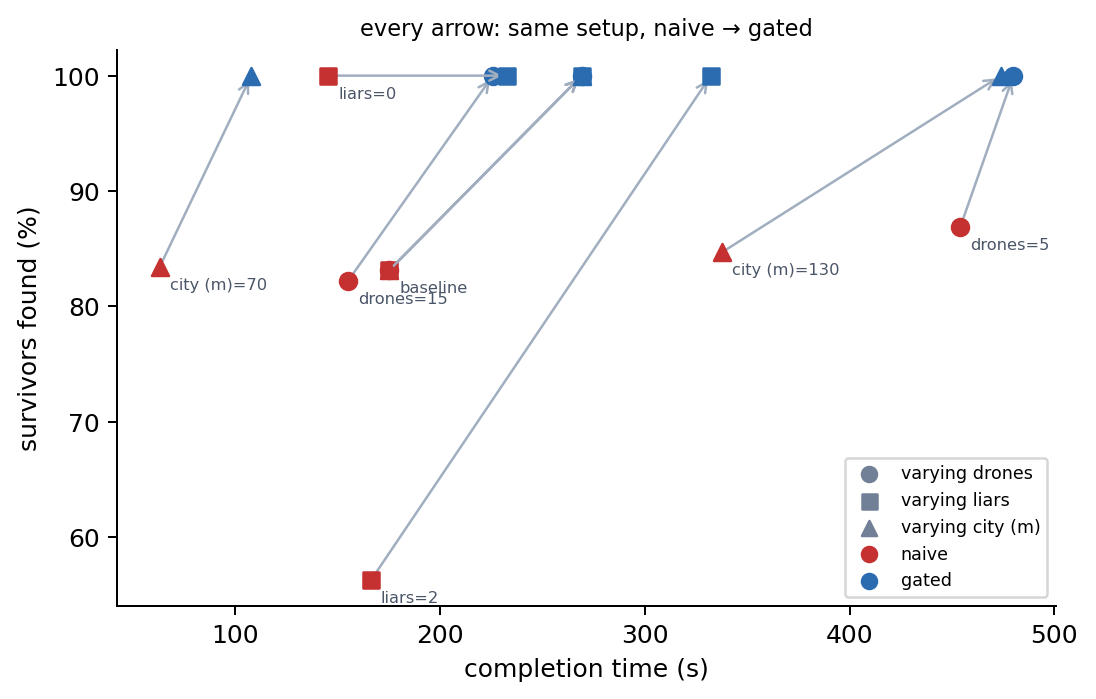
\includegraphics[width=0.78\linewidth]{Figures/results/sweep_tradeoff.png}
    \caption[The trade-off: survivors vs.\ time]{The trade-off. Each arrow joins the naive (red) and gated (blue)
    fleet on the same setting. Only the no-liar setting starts at 100\%.}
    \label{fig:sweep-tradeoff}
\end{figure}

\textbf{Identifying the liar.} The liar was identified in all 120 gated runs that contained one, with \textbf{no false
accusation} in any run. The first proof came a median 0.7--6.7\,s after the lie started, depending on the setting
(\autoref{tab:detection}). The range check R1 fired first in 76 runs, the speed check R2 in 32, an audit (R5) in 9 and the
camera (R4) in 3. In most settings every honest drone knew the liar within a fraction of a second of the first proof:
corroborating evidence spreads as fast as gossip. With only 5 drones, or 15 drones spread thinly, the second
independent proof that Corollary~\ref{cor:framing} requires takes longer to appear.

\begin{table}[!htbp]
\centering
\renewcommand{\arraystretch}{1.18}
\begin{tabular}{@{}l c c c c c c@{}}
\toprule
 & 5 drones & base & 15 drones & 2 liars & 70\,m & 130\,m \\
\midrule
Liar caught (gated)       & 20/20 & 20/20 & 20/20 & 20/20 & 20/20 & 20/20 \\
First proof (median, s)   & 12.9  & 14.6  & 18.9  & 14.4  & 15.5  & 13.1 \\
All honest know (median, s) & 38.6 & 14.8 & 24.6  & 14.7  & 15.7  & 13.8 \\
First rule (R1/R2/R4/R5)  & 15/5/0/0 & 13/7/0/0 & 13/2/2/3 & 10/10/0/0 & 10/3/1/6 & 15/5/0/0 \\
\bottomrule
\end{tabular}
\caption[Sweep: liar identification]{Liar identification in the sweep (the liar starts lying at 12.2\,s). In the
two-liar setting, ``caught'' means at least one liar proven. Zero false accusations in all 280 runs.}
\label{tab:detection}
\end{table}

\subsubsection{Four Fleets: Is the Price in \emph{Who} or in \emph{Where}?}
\label{sec:res-e1}

E1 adds the two reference fleets on 30 new districts, with the fair gate for every fleet (\autoref{fig:e1}).

\begin{figure}[!htbp]
    \centering
    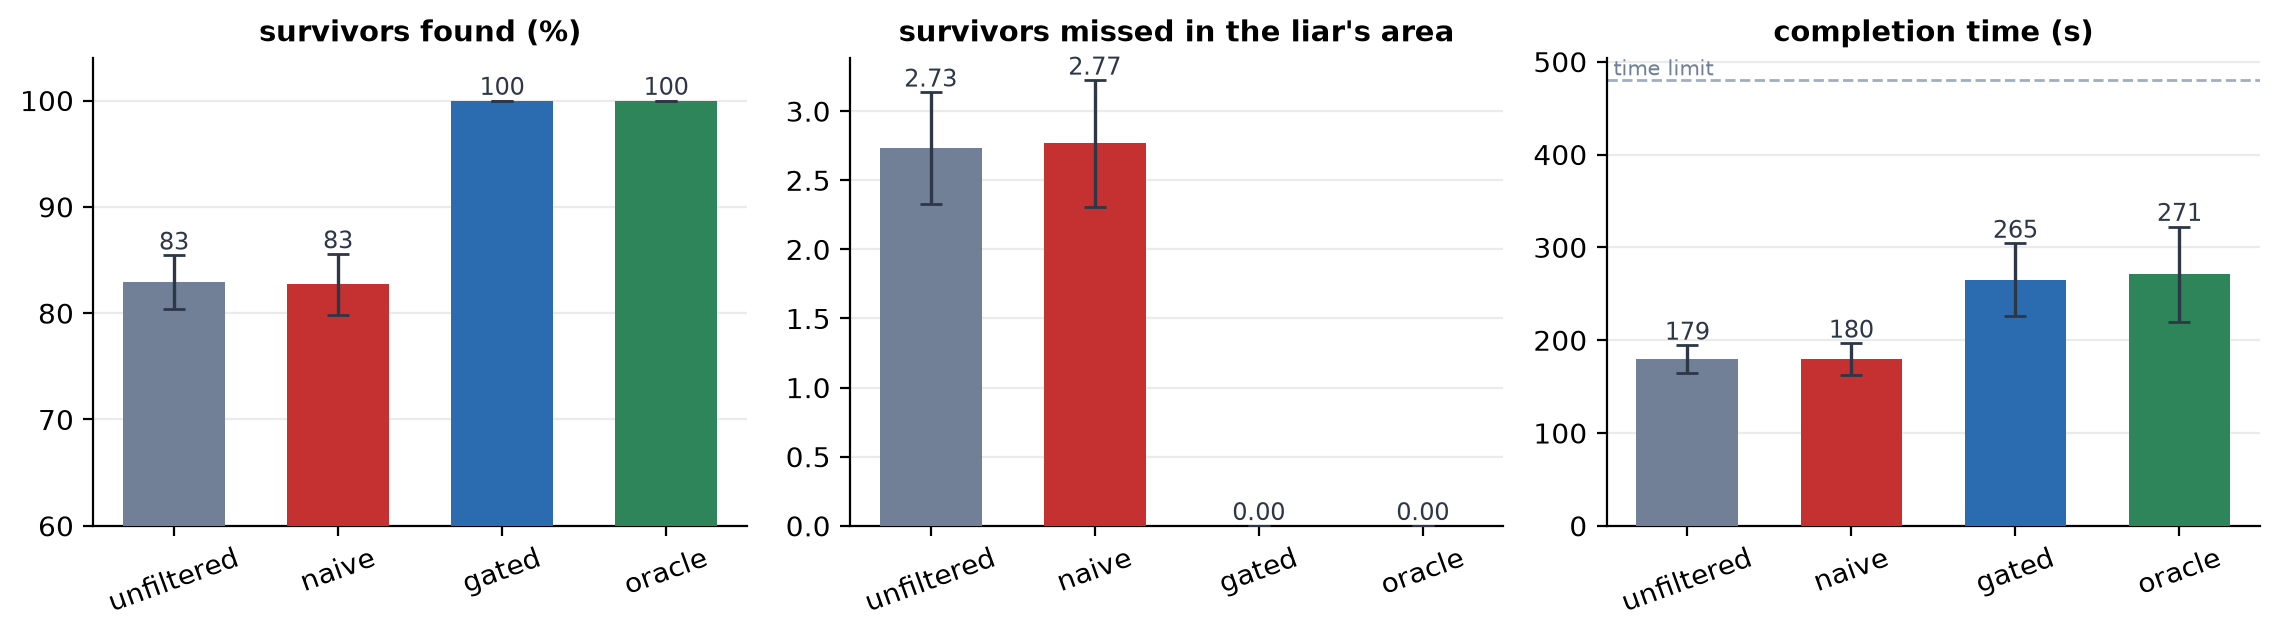
\includegraphics[width=\linewidth]{Figures/results/report_e1_fleets.png}
    \caption[E1: four fleets on 30 districts]{E1: the four fleets on 30 paired districts with one range-aware liar
    (95\% intervals). There were no collisions in any of the 120 runs.}
    \label{fig:e1}
\end{figure}

\begin{findingbox}[Finding 2: filtering alone buys nothing in the search, and the price of caution is not ignorance of the liar's identity]
\begin{itemize}
    \item \textbf{W-MSR does not help the search.} The naive fleet ($82.7\pm2.9\%$ found) is indistinguishable from
          the completely unfiltered fleet ($82.9\pm2.5\%$). Both miss survivors in all 30 districts, on average
          2.8 inside the liar's corner, because the damaging lie is a claim, and claims cannot be filtered.
    \item \textbf{Knowing beats filtering.} The gated fleet finds 100\% in all 30 districts ($p=1.5\times10^{-6}$ vs.\ naive)
          and knows the liar within $15.9\pm1.3$\,s.
    \item \textbf{The gated fleet matches the oracle.} The oracle, told the liar at $t=0$, is \emph{no faster}
          (271 vs.\ 265\,s, $p=0.94$). The time the gated fleet spends is spent on caution about \emph{where} drones may
          be, not on finding out \emph{who} lies. Once the liar is known, the gated fleet behaves exactly like the oracle.
\end{itemize}
\end{findingbox}

\subsubsection{Which Liars are Caught? (E2)}
\label{sec:res-e2}

E2 varies the kind of lie: three ways of faking a position (\emph{fake sweep}, a blunt fake trajectory over the corner;
\emph{range-aware}, which matches every listener's range where geometry allows; \emph{radio shadow}) and a liar that
flies its \emph{true} position and lies only about coverage. Each is crossed with two ways of claiming: the whole
corner at once, or cell by cell as its (fake) sweep passes. The results are in \autoref{fig:e2} and
\autoref{tab:e2}.

\begin{figure}[!htbp]
    \centering
    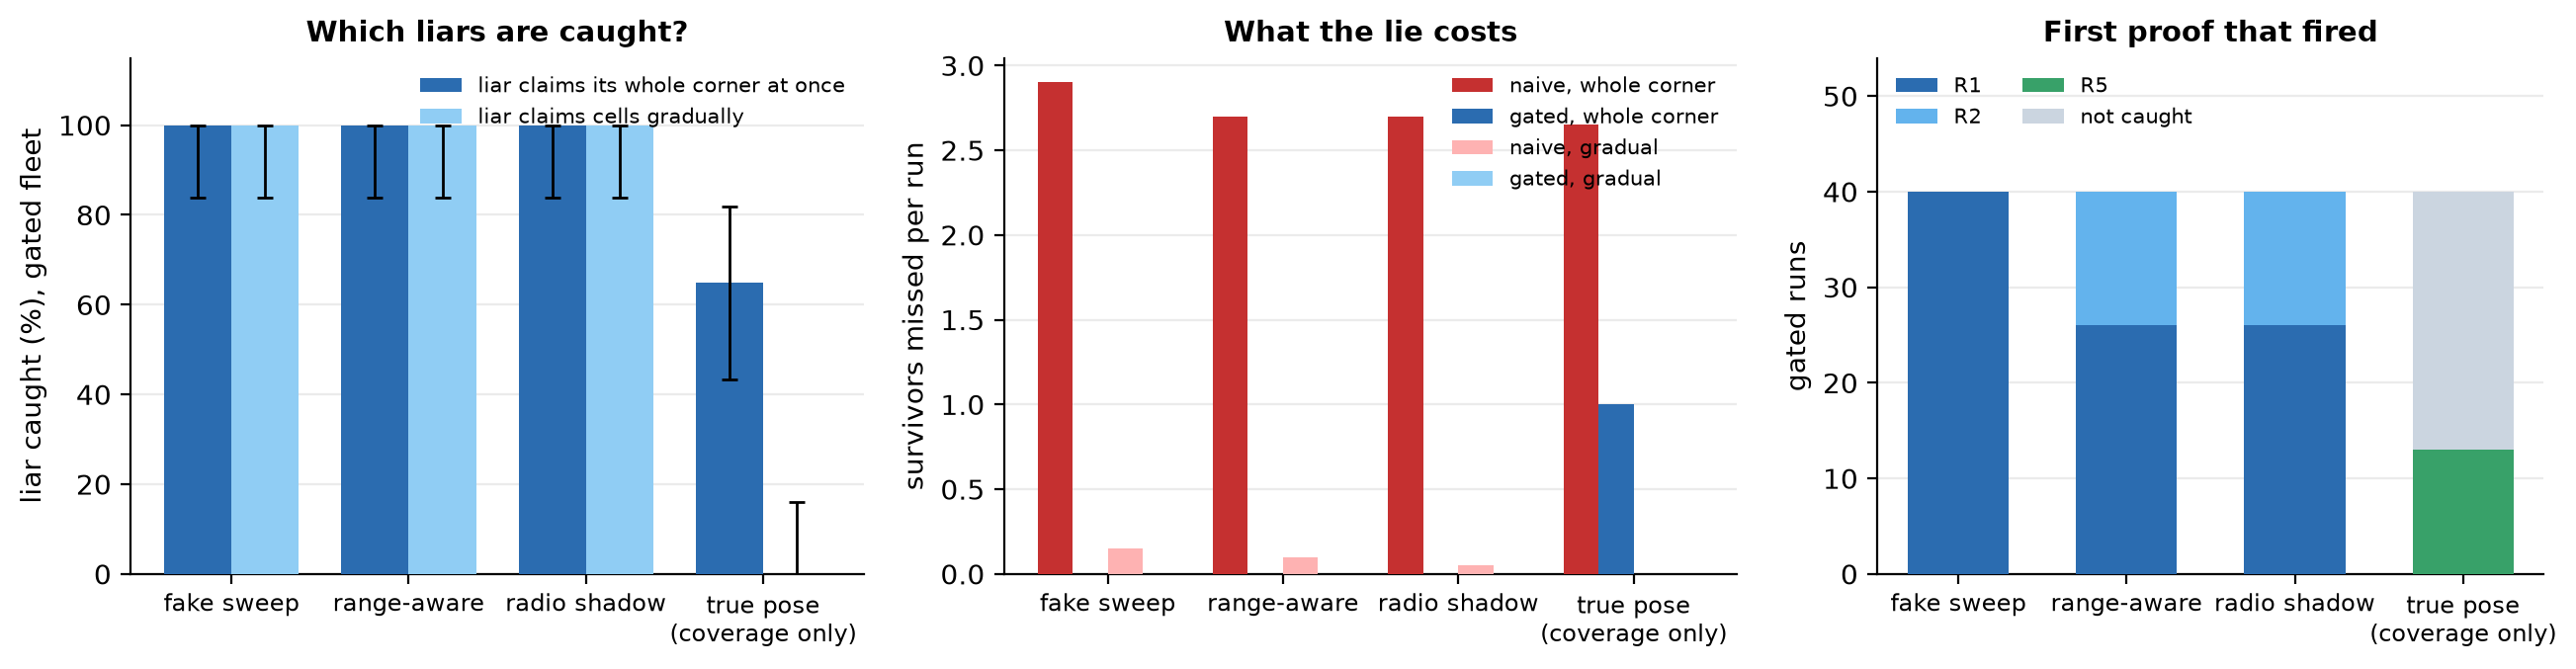
\includegraphics[width=\linewidth]{Figures/results/report_e2_detection.png}
    \caption[E2: detection by liar type]{E2: catch rate of the gated fleet with 95\% Wilson intervals (left), survivors
    missed per run (middle; bars at zero are not drawn), and the first proof that identified the liar (right; 40
    gated runs per liar type).}
    \label{fig:e2}
\end{figure}

\begin{table}[!htbp]
\centering
\renewcommand{\arraystretch}{1.18}
\begin{tabular}{@{}l l c c c c@{}}
\toprule
\textbf{Position lie} & \textbf{Claims} & \textbf{Caught} & \textbf{First proof / all know (s)} &
\multicolumn{2}{c}{\textbf{Survivors found (\%)}} \\
\cmidrule(lr){5-6}
 & & (gated) & (median) & naive & gated \\
\midrule
fake sweep   & whole corner & 20/20 & 12.3 / 12.5 & 81.9 & \textbf{100} \\
             & gradual      & 20/20 & 12.3 / 12.5 & 99.1 & \textbf{100} \\
range-aware  & whole corner & 20/20 & 14.6 / 14.8 & 83.1 & \textbf{100} \\
             & gradual      & 20/20 & 14.6 / 14.8 & 99.4 & \textbf{100} \\
radio shadow & whole corner & 20/20 & 14.7 / 14.9 & 83.1 & \textbf{100} \\
             & gradual      & 20/20 & 14.7 / 14.9 & 99.7 & \textbf{100} \\
true pose (coverage only) & whole corner & 13/20 & 33.1 / 44.1 & 83.4 & 93.8 \\
             & gradual      & 0/20  & -- & 100 & 100 \\
\bottomrule
\end{tabular}
\caption[E2: detection results]{E2 results (20 paired seeds per row; lying starts at 12.2\,s). No false
accusation occurred in any of the 320 runs.}
\label{tab:e2}
\end{table}

\begin{findingbox}[Finding 3: a position lie is caught at once; a pure coverage lie only by audits]
\begin{itemize}
    \item \textbf{Every liar that fakes its position is caught}, in 120 of 120 runs, a median 0.1--2.5\,s after it
          starts lying. Even the range-aware liar cannot hide: whenever three listeners surround it, or it moves faster
          than a drone can fly to keep its story consistent, R1 or R2 fires.
    \item \textbf{The damage comes from claiming a large area.} A liar that claims its whole corner costs the naive
          fleet 2.7--2.9 survivors per run. A liar that claims cells only along its fake path costs almost nothing
          (0.05--0.15), because overlapping honest cameras re-view most of those cells anyway.
    \item \textbf{A coverage-only liar is the hard case.} It is caught only by an audit (R5), in 13 of 20 runs, a
          median 21\,s after the lie. Whenever it was caught, the gated fleet found everyone. In the 7 runs where the
          audits missed it, the gated fleet lost 1--5 survivors, as many as the naive fleet. When the same liar claims
          gradually it is never caught, but it is then also harmless: both fleets found every survivor.
\end{itemize}
\end{findingbox}

\textbf{A safety weakness exposed by E2.} All 22 collisions of E2 occurred against the blunt \emph{fake sweep} liar,
which hovers in place while claiming to be far away: 16 in 12 of 40 gated runs, and 6 in 5 of 40 naive runs. No other
liar type caused any. Two affected gated runs, re-flown with full logging, reproduced exactly: every collision was an
honest gated drone touching the hovering liar, 70--85\,s after the liar had been proven. A proven liar's beacons no
longer count as positions, and the range-shell check that replaces them probes only along the direction of motion
(\autoref{sec:limitations}), so a drone re-sweeping the reopened corner can drift into a liar it has not just sighted.
The range-aware liar is unaffected because its claimed position stays close to its real one. Checking the whole
reachable shell, as in the extended gate of \autoref{sec:res-collision}, is the clearest target for future work.

\subsubsection{The Caution Knob: Audit Fraction (E3)}
\label{sec:res-e3}

E3 targets the hardest case from E2, the coverage-only liar that claims its whole corner, and varies the audit
fraction $q$ over 30 districts (\autoref{fig:e3}).

\begin{figure}[!htbp]
    \centering
    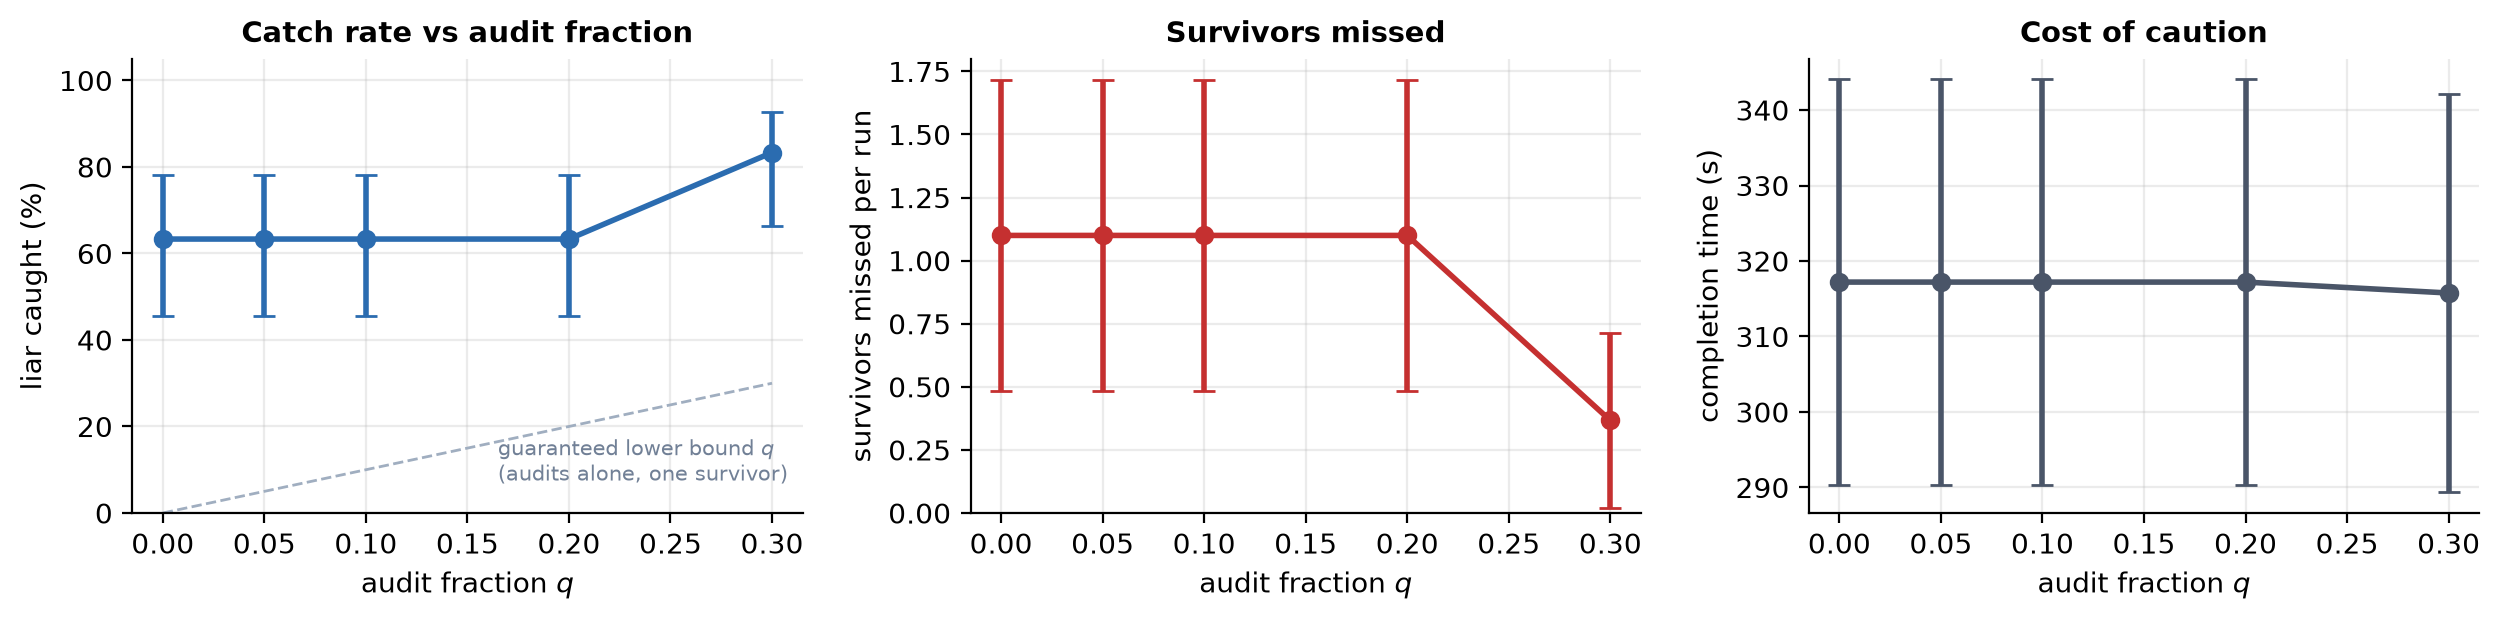
\includegraphics[width=\linewidth]{Figures/results/report_e3_audit.png}
    \caption[E3: the audit fraction]{E3: catch rate (95\% Wilson intervals), survivors missed and completion time against
    the audit fraction $q$, for a liar that flies its true position and lies only about coverage (30 paired districts
    per value). The dashed line is the guarantee of Proposition~\ref{prop:audit} for deliberate audits alone. Only
    9--11 of 30 runs per value finished within the 360\,s limit, so the time panel cannot resolve the cost of $q$.}
    \label{fig:e3}
\end{figure}

\begin{findingbox}[Finding 4: overlapping cameras audit for free; deliberate audits matter only above that level]
\begin{itemize}
    \item With $q=0$, i.e.\ no deliberate audits at all, the liar is still caught in 63\% of runs (19/30). Honest
          drones' cameras overlap at region borders and incidentally view cells the liar claimed. A survivor seen in
          such a cell is a proof (R5), whoever looked.
    \item Up to $q=0.2$ nothing changes. The audit budget $\lceil q\,n_j\rceil$ is already met by those incidental
          views, so no extra cell is visited, and the 30 runs come out identical for every $q\le0.2$.
    \item At $q=0.3$ the budget exceeds the free overlap. The catch rate rises to 83\% (25/30), and survivors missed
          fall from $1.10\pm0.62$ to $0.37\pm0.35$ per run. The measured catch rates stay well above the guaranteed lower
          bound of Proposition~\ref{prop:audit}.
\end{itemize}
\end{findingbox}

The practical lesson is that $q$ should be set relative to the \emph{free} audit rate of the fleet geometry. Below it,
audits cost nothing and add nothing. Above it, every extra percent of audits buys a measurable increase in the chance
of exposing a coverage-only liar.

\subsubsection{A Liar Hiding in the Flight Path}
\label{sec:res-collision}

The quantitative experiments use a passive liar. To illustrate the safety side of the gate, we also recorded a stress
demonstration: the liar claims to sweep its far corner while waiting, still, in the path of honest drones, 0.6\,m above
the height the camera covers. This liar and the extended gate (which checks the whole reachable cone of the range shell)
are an experimental extension outside the evaluated code, so the replay is an illustration only
(\autoref{fig:collision}). The naive fleet, believing the fake position, flew into the liar six times and missed three
survivors. The gated fleet, treating a possible liar as ``somewhere on its range sphere'', had no collision, knew the
liar by 12.5\,s and found all 16 survivors, at the price of a longer mission (365 vs.\ 212\,s).

\begin{figure}[!htbp]
    \centering
    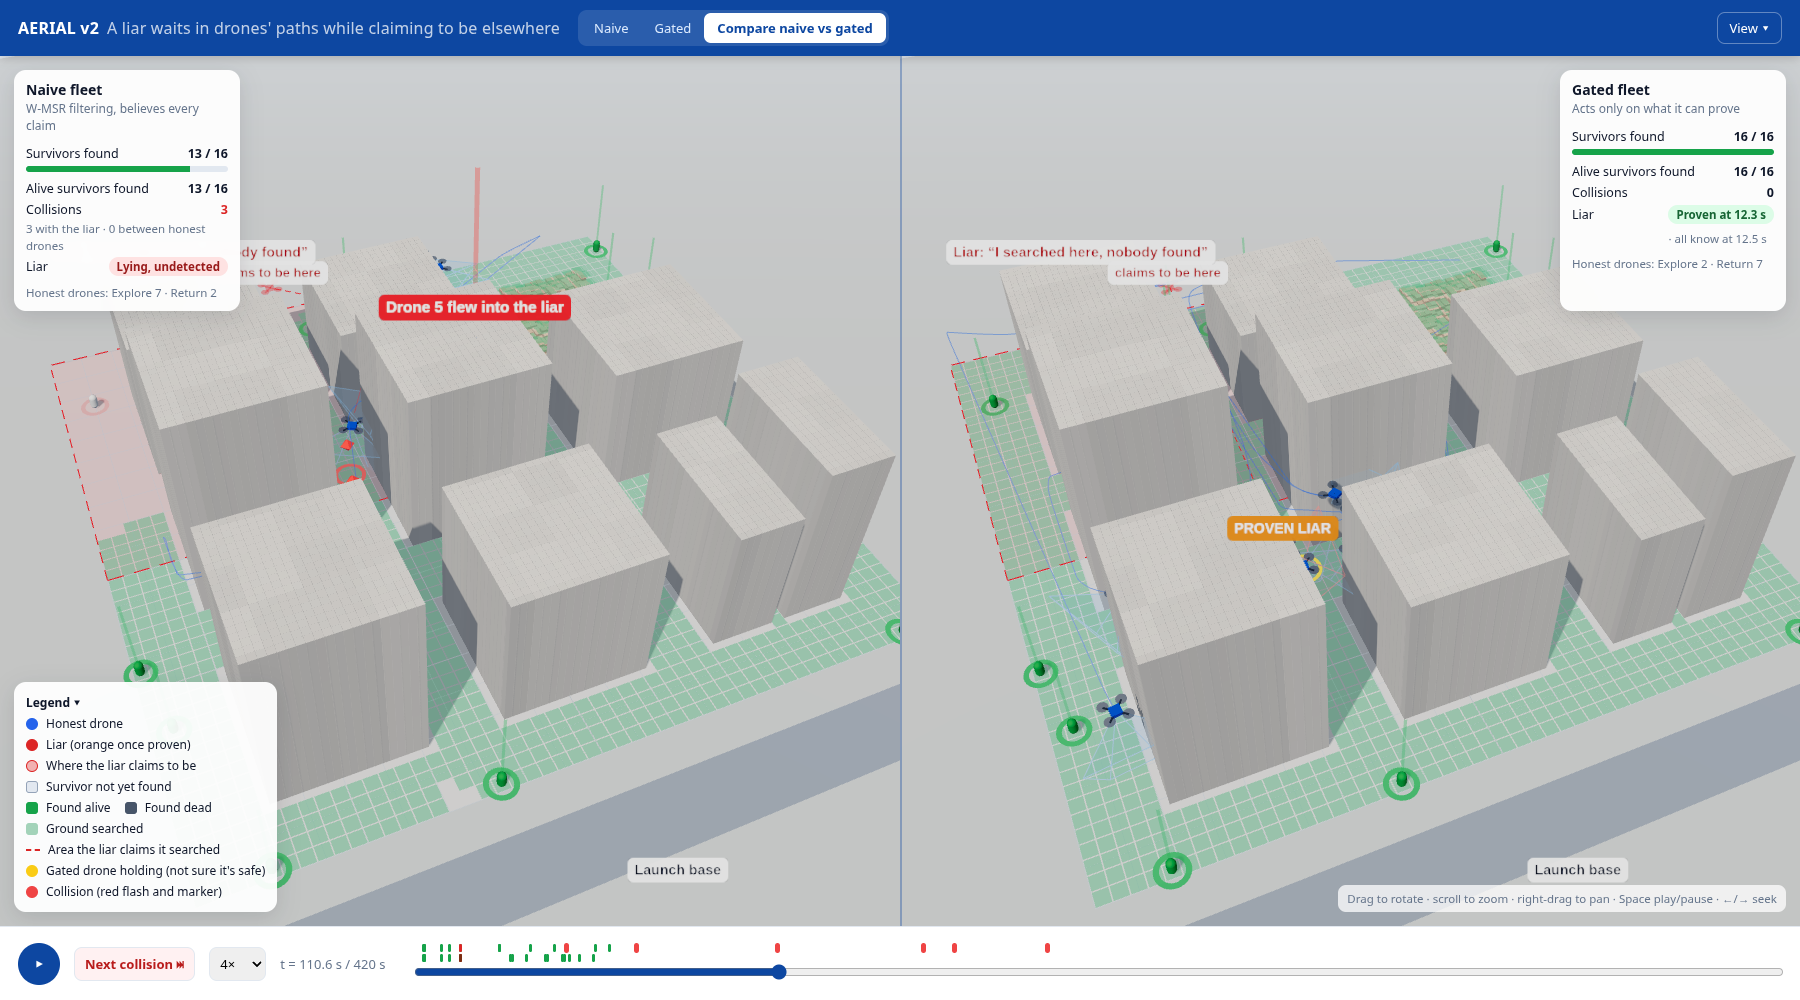
\includegraphics[width=\linewidth]{Figures/results/replay_collision.png}
    \caption[Illustration: naive drones fly into a hidden liar]{Illustration (experimental liar extension): at
    110.6\,s a naive drone flies into the liar (left), which it believes to be elsewhere. The gated drones keep their
    distance from the liar's range sphere and from its camera-located position (right).}
    \label{fig:collision}
\end{figure}

\subsubsection{Resilient Survivor Localisation}
\label{sec:res-localisation}

Where numbers \emph{are} involved, W-MSR does its job (\autoref{fig:localisation}). When one of 2--8 observers reports a
survivor's position offset by up to 20\,m, the plain mean is dragged by almost the full lie (19.8\,m of a 20\,m lie with
5 observers). W-MSR stays within 0.2--0.7\,m of the truth for every lie size. The price appears when nobody lies: W-MSR
discards honest data and has 0.2--0.45\,m error, against almost zero for the mean.

\begin{figure}[!htbp]
    \centering
    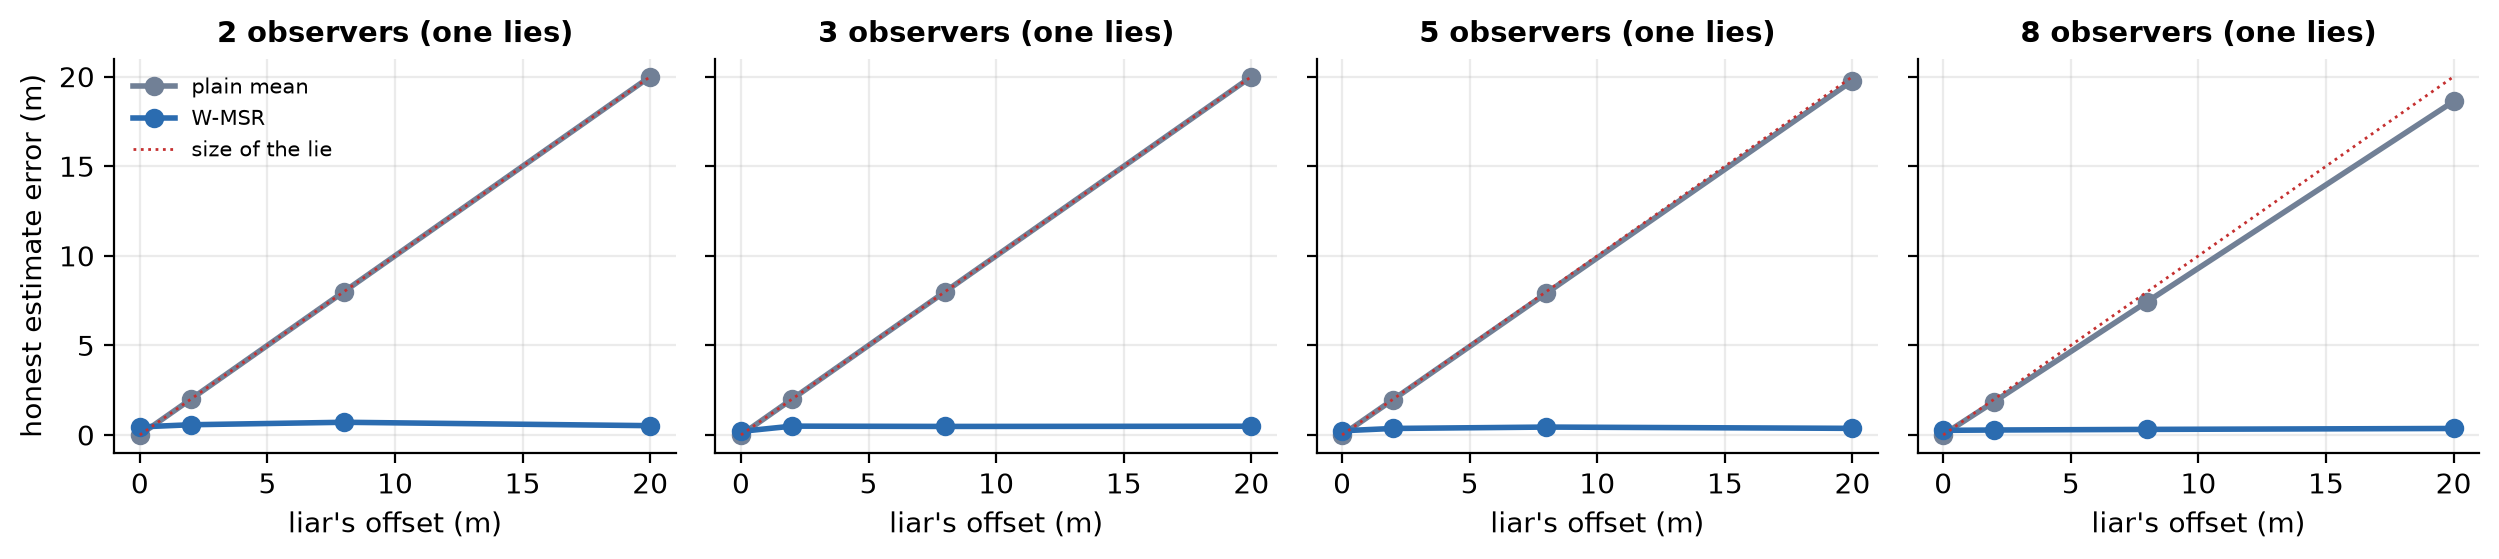
\includegraphics[width=\linewidth]{Figures/results/report_localisation.png}
    \caption[Survivor localisation: W-MSR vs.\ mean]{Error of the honest drones' combined estimate of a survivor's
    position when one observer lies by a given offset.}
    \label{fig:localisation}
\end{figure}

\subsubsection{Theory Studies from the 2D Build}
\label{sec:res-theory}

A first, simpler 2D build of the project (fixed-topology formation flight) was used to check the network theory behind
the fleet. Its studies (\autoref{fig:lambda2}, \autoref{fig:er}, \autoref{fig:degradation}) support three statements
used in the main system:

\begin{enumerate}
    \item \textbf{Algebraic connectivity predicts convergence} (480 runs). The convergence rate grows with $\lambda_2$
          and then saturates at the limit set by the controller gains. Predicted from the whole Laplacian spectrum, it
          is accurate to within 1.7\% mean error without packet loss. Under 30\% packet loss, using $\lambda_2$ alone
          gives 70\% error, so the full spectrum is needed.
    \item \textbf{$(2F+1)$-robustness is sufficient, not necessary} (4,860 runs on Erd\H{o}s--R\'enyi graphs). When the
          condition held, W-MSR succeeded in all 1,428 runs with $F=1$. When it failed, only 32\% of 1,002 runs
          succeeded, and the unfiltered mean succeeded in 5\% overall.
    \item \textbf{W-MSR collapses as soon as liars exceed $F$, and costs information when nobody lies.} Success is
          100\% while the actual number of liars is at most the assumed $F$, then falls sharply. With nobody lying,
          W-MSR discards 29\% ($F=1$) and 51\% ($F=2$) of honest messages.
\end{enumerate}

A 14,400-run trade-off study in the same build (four attacks, packet loss, gate horizon and margin) found the same
pattern as the 3D sweep. The gated fleet violated the STL safety requirement in 1.5\% of runs, against 99.9\% for the
naive fleet. The oracle fleet gained nothing over the gated fleet, again because the price is where the liar might be,
not who it is.

\begin{figure}[!htbp]
    \centering
    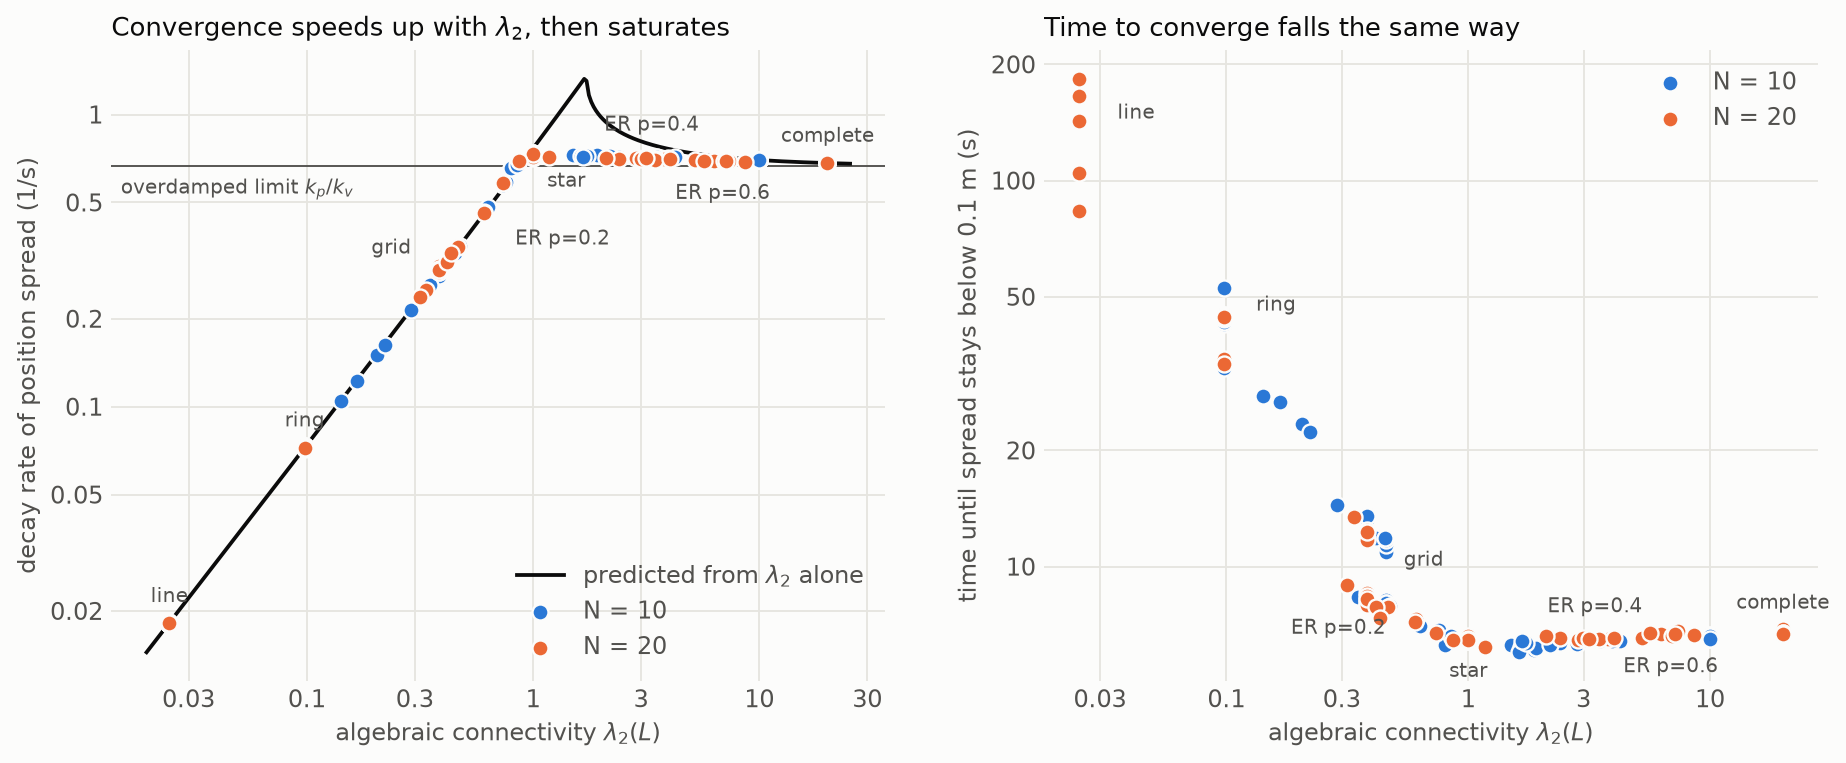
\includegraphics[width=\linewidth]{Figures/results/lambda2_convergence.png}
    \caption[2D study: convergence vs.\ algebraic connectivity]{2D study: consensus convergence rate (left) and time
    to converge (right) against the algebraic connectivity $\lambda_2$, for six topologies and Erd\H{o}s--R\'enyi graphs.}
    \label{fig:lambda2}
\end{figure}

\begin{figure}[!htbp]
    \centering
    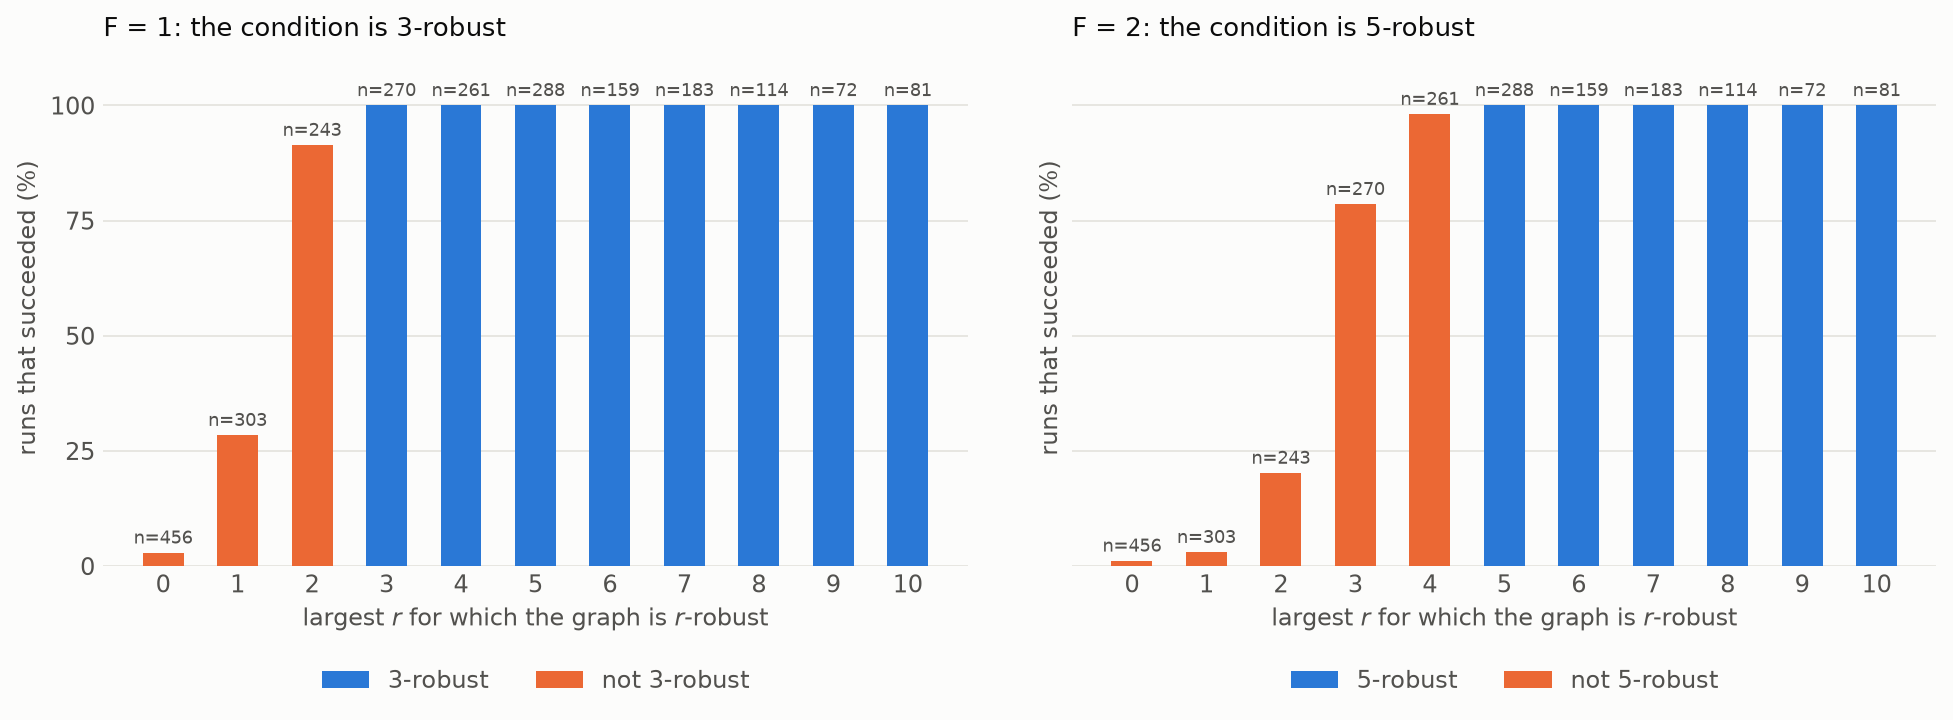
\includegraphics[width=\linewidth]{Figures/results/er_robustness.png}
    \caption[2D study: W-MSR success vs.\ network robustness]{2D study: W-MSR success on Erd\H{o}s--R\'enyi graphs
    against the graph's robustness (blue: the sufficient condition holds).}
    \label{fig:er}
\end{figure}

\begin{figure}[!htbp]
    \centering
    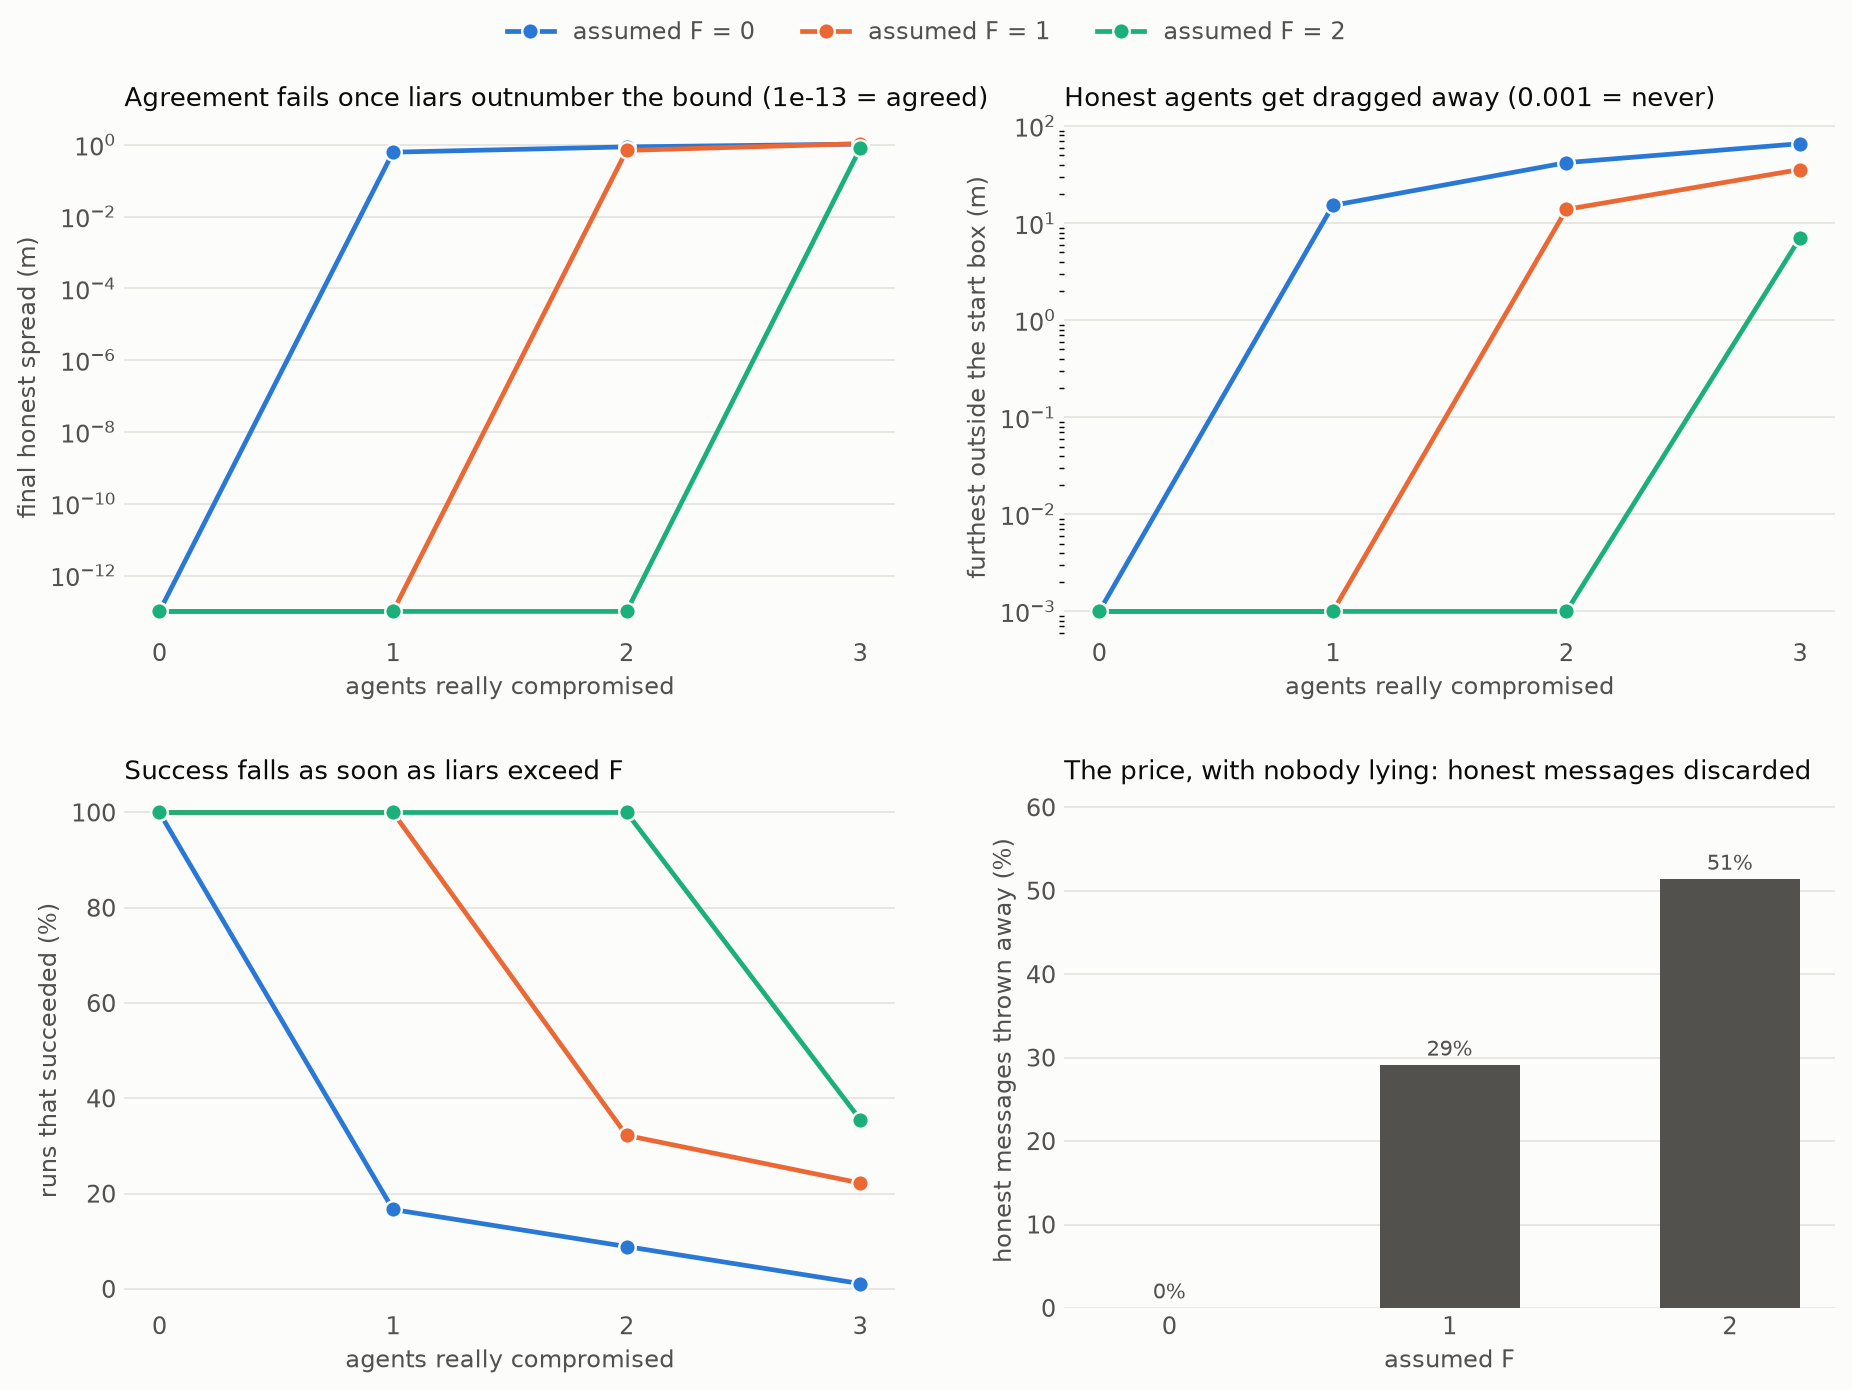
\includegraphics[width=0.85\linewidth]{Figures/results/degradation.png}
    \caption[2D study: graceful degradation of W-MSR]{2D study: what happens when the actual number of liars exceeds
    the assumed $F$ (top, bottom left), and the information W-MSR throws away when nobody lies (bottom right).}
    \label{fig:degradation}
\end{figure}

\FloatBarrier
\section{Limitations}
\label{sec:limitations}

Each limitation below bounds what the results above can claim.

\textbf{Performance.}
\begin{itemize}
    \item \textbf{Caution costs time}: about $+90$\,s at the baseline, \emph{even with no liar}. With a small fleet or
          a large city, the gated fleet often does not finish within 480\,s, so its true time there is underestimated.
    \item \textbf{Coverage-only liars are caught only by audits}, and audits are probabilistic
          (Proposition~\ref{prop:audit}); see E2 and E3.
\end{itemize}

\textbf{Model.}
\begin{itemize}
    \item Signed messages without equivocation, range noise bounded by 0.2\,m (real UWB has rare outliers, which would
          require a robust version of R1), static 2.5D terrain without overhangs, point drones, and no wind.
    \item \textbf{Terrain contact.} Drones are points and the terrain is a 1\,m raster. In the sweep, honest drones of
          both fleets occasionally grazed a wall: a 1\,Hz trajectory sample fell inside a building's outermost 1\,m
          cell in 56 of 140 naive and 69 of 140 gated runs. In 97\% of these cases the drone was at most 1\,m inside
          and only for a single sample (the worst case was 5\,m). These contacts are excluded from the collision
          counts, which count drone pairs only. A body radius and a terrain term in the gate would remove them.
    \item A liar that deliberately rams other drones (Assumption A8) defeats any gate that controls only the honest
          drone's own motion. This is out of scope.
\end{itemize}

\textbf{Method.}
\begin{itemize}
    \item The gate's check against a possible liar's range shell is analytic and probes only along the direction of
          motion. Against a hovering liar that claims to be far away, this let gated drones touch the liar in 12 of 40
          E2 runs (\autoref{sec:res-e2}). A possible liar whose latest packet was lost is covered only by the silence
          rule.
    \item ``Done'' uses belief plus audits. The fraction of \emph{known}-cleared cells is reported but not required for
          landing.
    \item Planned but not built: a rule R7 for coverage claims that are impossible from the liar's true path,
          heading-based altitude layers (layers are assigned by drone id), a consensus-based regroup at the base, and
          full 3D detours.
\end{itemize}

\textbf{Evaluation.}
\begin{itemize}
    \item All results are from simulation, with 20--30 seeds per configuration. The demonstrations use one seed each,
          and the collision replay uses an experimental liar extension that is not part of the evaluated code.
\end{itemize}
